\documentclass[11pt]{article}
\usepackage[margin=1in]{geometry}
\usepackage{amsmath,amssymb}
\usepackage{graphicx}
\usepackage{booktabs}
\usepackage[colorlinks=true,linkcolor=blue,citecolor=blue,urlcolor=blue]{hyperref}
\newcommand{\ueV}{\,\mu\mathrm{eV}}
\title{Majorana zero modes in silicon: quantified constraints on the conduction band\\
and a conditional hole-based route}
\author{W.~T.~Trevena}
\date{June 2026 --- draft v4}
\begin{document}
\maketitle

\begin{abstract}
We present a computational feasibility and falsification study of Majorana
zero modes in silicon nanowires (Bogoliubov--de Gennes, valley-resolved,
six-band $k\cdot p$ + Poisson; every quoted number regenerates from the
public repository and is machine-verified against its numerical ledger).
\emph{Conduction band}: three quantified obstructions --- a spin--orbit
shortfall, the single-channel $g \approx 2$ Zeeman ceiling, and valley
physics, where we prove smooth interfaces benign under inter-valley pairing
but find each atomic step acts as a near-$\pi$ Josephson junction
($\Delta\varphi \approx 0.85\pi$) that caps the gap at $\sim$18\% from the
first step. With miscut-derived step ensembles, device \emph{yield} is the
binding statistic: 2--5\% for unaligned wires even on premium wafers,
50--68\% for wires within $10^\circ$ of step edges. Within this model
class, conduction-band Si is strongly disfavored unless step morphology is
specifically controlled. \emph{Valence band}: holes evade valley physics;
our six-band [110]-channel treatment (the orientation of every benchmark
device) resolves the long-standing model-vs-experiment $g$ discrepancy as
predominantly an axes artifact and yields gate-stable
$g_{x'} = 1.4$--$1.7$, $m^* \approx 0.20$, $\alpha$ up to
0.075\,eV\,\AA. Adjudicated against explicit operational tiers with the
dynamic tunneling self-energy as the central estimate (static values are
upper bounds): measured thick Si:B reaches 8--10$\ueV$ at tilted field
(marginal detection tier); hypothetical$^\dagger$ Pauli-limited thin-film
Si:B, $\sim$13$\ueV$; hypothetical$^\dagger$ hard-gap Al/Si-hole,
17--18$\ueV$ (the only scenario approaching the nonlocality tier and
surviving quasiparticle poisoning at realistic temperatures). The binding
materials constraint is correlated electrostatic disorder: calibrated
against oxide-interface charge, standard trap densities produce potential
disorder orders of magnitude beyond tolerance, so interface quality ---
not step morphology or parent choice --- gates any MOS-style silicon
implementation. Two measurements would do the most to settle the platform:
the parallel critical field of thin Si:B films and the device-geometry
[110] hole $g$-tensor. Qubit relevance is not established.
\end{abstract}

\section{Introduction}
Semiconductor--superconductor hybrid nanowires remain the most studied route to MZMs
\cite{kitaev,lutchyn2010,oreg2010}, and a decade of experiments---from the first InSb
signatures \cite{mourik} through the disorder-driven retractions and reappraisals
\cite{pan2020} to protocol-based standards \cite{aghaee}---has made one lesson clear:
material quality and honest accounting of trivial explanations dominate the problem.
Silicon, the most controllable semiconductor in existence, has been conspicuously
absent from this program, for reasons usually stated qualitatively: weak spin--orbit
coupling (SOC), a small $g$-factor, and conduction-band valley degeneracy.

This paper is a computational feasibility and falsification study: it makes
those reasons quantitative, finds that one of them hides a qualitatively new
failure mechanism, and shows that silicon \emph{holes} evade it --- while
facing their own multiband $g$-tensor, electrostatic, and parent-interface
constraints, quantified below. Our contributions: (i) a quantified electron verdict (Secs.~\ref{sec:soc},
\ref{sec:catch}); (ii) an exact unitary equivalence making smooth-interface valley
splitting benign under the physical inter-valley pairing channel, and the identification
of single-atomic interface steps as near-$\pi$ Josephson junctions that
sharply degrade protection from the first step (single-step cap $\sim$18\%) (Sec.~\ref{sec:valley}); (iii) a Luttinger--Kohn (LK)
derivation of the gate-field covariation of hole parameters, which erodes free-parameter
optimism but preserves a viable design (Sec.~\ref{sec:holes}); and (iv) orientation-
resolved feasibility maps for two silicon-compatible parents---laser-doped
superconducting Si:B \cite{bustarret,prb2010,chiodi2024,reviewSiSC} and Al
films---including thin-film design targets, metallization renormalization, and
quasiparticle-poisoning limits (Sec.~\ref{sec:parents}). Throughout, spectral
diagnostics are cross-checked by recursive-Green's-function transport
(Sec.~\ref{sec:transport}).

\section{Model and methods}
We use the standard single-channel BdG Hamiltonian
\begin{equation}
H = \left(\frac{\hbar^2 k^2}{2m^*} - \mu + V(x)\right)\sigma_0
+ \alpha k \sigma_z + E_Z \sigma_x \quad\text{(normal part)},\qquad
\Delta\, i\sigma_y \quad\text{(pairing)},
\end{equation}
discretized with exact particle--hole symmetry by construction, topological for
$E_Z^2 > \Delta^2 + \mu^2$. Validation (repository Fig.~1): gap closing at the analytic
boundary; end-localized zero modes; exponential length splitting; finite-wire vs
analytic bulk-gap agreement. Valley physics uses an $8N$ basis with \emph{inter-valley}
singlet pairing $\Delta(\nu_x \otimes i\sigma_y)$---the physical zero-momentum channel
since the relevant valleys are time-reversed partners---with arbitrary complex
valley-orbit (VO) profiles $\lambda(x)$ and a gauge-covariant phase-locked
Dresselhaus-type SOC option. Hole parameters derive from a four-band LK model of the
fin cross-section (validated against exact [100] bulk masses) with vertical field,
bare ($\kappa$) and orbital Zeeman terms. Transport uses a dimension-generic RGF with
Ando wave-matched normal leads and an $E=0$ reflection invariant $\mathrm{sign}\det r$
(kwant-equivalent; validated against closed-chain spectra to $10^{-13}$). A test suite
pins every exact claim. $\Delta$ is a \emph{static} induced gap (the
$\omega = 0$ limit of the standard tunneling self-energy); parent-gap field
suppression enters via $\Delta_{ind} \le \Delta_p(B)$ and metallization via the
quasiparticle weight $Z$ \cite{cole2015,maier,reeg} (Supplement S6); the full
dynamical self-energy is solved as a control in Sec.~\ref{sec:controls} and
validates the static-$Z$ treatment directionally while lowering its numbers
by 24--30\%. All caricature choices (GL/Zeeman-linear parent gaps, iid
onsite disorder with correlation length $dx$, hard-wall LK geometry) are stated
where used; complete per-figure parameter tables, seed families, and
discretization/length/seed/grid convergence studies are in Supplement S4--S5.
Throughout, claims carry one of three epistemic levels, stated where
ambiguity is possible: \emph{exact within model} (the valley equivalence
theorem, the $g = 2$ ceiling, topological criteria), \emph{numerical within
model} (gap optimizations, step ensembles, disorder thresholds, transport),
and \emph{device extrapolation} (parent feasibility, interface assumptions,
fabrication design rules).

% ============================================================================
% drafts/usable_criterion.tex  (R5-5, drafting only -- to be integrated)
% Operational definition of "usable" demanded by referee round 5, plus a
% decision table evaluating the seven master-table rows against the tiers.
% Requires booktabs and the \ueV macro. All numbers traced to
% output/data/key_numbers.json tags (in comments) or committed text.
% ============================================================================
\subsection{Operational criteria}\label{sec:usable}
``Usable'' is not a single threshold; we therefore evaluate every platform
scenario of Table~\ref{t:scenario} against three named, quantitative tiers.

\paragraph{Tier S (spectroscopy/detection).} Topological gap
$\Delta_{\mathrm{top}} \ge 2 k_B T_{\mathrm{eff}}$ at
$T_{\mathrm{eff}} = 50$\,mK, i.e.\ $\Delta_{\mathrm{top}} \ge 8.6\ueV$
($k_B \times 50\,\mathrm{mK} = 4.3\ueV$), \emph{and} Majorana splitting
$E_0 \le 0.1\ueV$ at $L \le 3\,\mu$m. The gap threshold ensures the
subgap feature is resolvable against thermal smearing in tunneling
spectroscopy at a routinely achieved electron temperature; the splitting
threshold keeps the zero-bias peak unsplit at spectroscopic resolution and
is met by our clean finite-wire checks ($E_0 = 3\times10^{-4}\ueV$ at
$2\,\mu$m, repository Fig.~1; hole-wire check $E_0 \approx 0$ at $3\,\mu$m,
\texttt{fig8.hole\_wire\_finite\_check}).

\paragraph{Tier N (nonlocality/fusion).} Additionally
$\Delta_{\mathrm{top}} \ge 20\ueV$ and disorder half-gap threshold
$W_{1/2} \ge 200\ueV$. The $20\ueV$ value is the protection scale used
throughout this paper (e.g.\ the $\alpha$ requirement of
Sec.~\ref{sec:soc}, \texttt{fig3.alpha\_needed\_for\_20ueV}), giving
$\gtrsim 4\,k_BT$ headroom for braiding/fusion protocols at 50\,mK; the
disorder threshold demands a finite margin against realistic potential
fluctuations, against which the transport-level
$W_{1/2} \approx 548\ueV$ of the engineered-electron case
(Sec.~\ref{sec:transport}) and the hole-wire gap persisting to
$W \approx 300\ueV$ (\texttt{fig8.hole\_wire\_finite\_check}) are measured.

\paragraph{Tier Q (parity-coherent qubit).} Additionally a sustainable
parent quasiparticle fraction $x_{qp} \le 10^{-6}$ at
$T_{\mathrm{eff}} \ge 50$\,mK given the parent gap \emph{at the operating
field}: $10^{-6}$ is the standard parity-lifetime requirement, and 50\,mK
is the coldest electron temperature routinely demonstrated for
quasiparticle thermalization. From \texttt{qp\_poisoning.py}
(Supplement S7): the Si:B operating points ($\Delta_p(B^*) = 29$--$33\ueV$)
require $T_{\mathrm{eff}} \le 25$--29\,mK and therefore fail; the Al
reference ($\Delta_p = 150\ueV$ at 1\,T) requires only
$T_{\mathrm{eff}} \le 130$\,mK and passes.

% (decision table superseded by the scenario table t:scenario in the main text)

% ============================================================================
%% R5-5 LANGUAGE-SOFTENING LIST (for the lead session to apply to paper.tex)
%% Every sentence in paper.tex found using absolute language, with line
%% context and a suggested softened replacement. Line numbers refer to the
%% committed paper.tex at review round 5.
%%
%% 1. Line 7 (title): "Majorana zero modes in silicon: quantified failure of
%%    the conduction band and a conditional hole-based route"
%%    -> "Majorana zero modes in silicon: quantified constraints on the
%%    conduction band and a conditional hole-based route"
%%
%% 2. Line 18 (abstract): "Conduction-band wires fail independently on three
%%    axes: ..."
%%    -> "Conduction-band wires face three independent, quantified
%%    obstructions: ..."
%%
%% 3. Lines 20-21 (abstract): "a $g\!=\!2$ ceiling forbidding induced gaps
%%    above $116\ueV$ at attainable fields"
%%    -> "a $g\!=\!2$ ceiling that, within our single-channel model, prevents
%%    induced gaps above $116\ueV$ from reaching the topological phase at
%%    attainable fields"
%%
%% 4. Lines 41-43 (abstract): "The hole route is therefore a \emph{conditional}
%%    feasibility result, decided by two standard measurements, not an
%%    established platform."
%%    -> "The hole route is therefore a \emph{conditional} feasibility result
%%    whose status two standard measurements would largely settle; it is not
%%    an established platform."
%%
%% 5. Lines 47-49 (abstract): "Two measurements decide the platform: the
%%    parallel critical field of thin Si:B films, and the wire-axis hole
%%    $g$-tensor in device geometry."
%%    -> "Two measurements would most sharply constrain the platform: the
%%    parallel critical field of thin Si:B films, and the wire-axis hole
%%    $g$-tensor in device geometry."
%%
%% 6. Lines 62-63 (intro): "This paper makes those reasons quantitative, finds
%%    that one of them hides a qualitatively new failure mechanism, ..."
%%    -> "... hides a qualitatively new obstruction ..."
%%
%% 7. Lines 66-68 (intro): "...the identification of single-atomic interface
%%    steps as near-$\pi$ Josephson junctions that destroy protection from
%%    the first step"
%%    -> "...as near-$\pi$ Josephson junctions that sharply degrade
%%    protection from the very first step (single-step cap: 18\% of the
%%    clean gap in our model)"
%%
%% 8. Line 107 (section title): "\section{Conduction band: three independent
%%    failures}"
%%    -> "\section{Conduction band: three independent obstructions}"
%%
%% 9. Lines 110-112: "below dilution-fridge protection scales and destroyed
%%    by any realistic disorder."
%%    -> "below dilution-fridge protection scales and removed by onsite
%%    disorder well below the modeled thresholds (Sec.~5)."
%%
%% 10. Lines 124-125: "any induced gap $\Delta \ge 116\ueV$ can never reach
%%     the topological phase at attainable fields"
%%     -> "any induced gap $\Delta \ge 116\ueV$ cannot reach the topological
%%     phase for $B \le 2$\,T within the single-channel $g=2$ model"
%%
%% 11. Line 168: "holes are immune by construction."
%%     -> "holes, which have no conduction-band valleys, are not subject to
%%     this mechanism within our model."
%%
%% 12. Line 266 (discussion): "Two measurements now decide the silicon
%%     question."
%%     -> "Two measurements would now do the most to settle the silicon
%%     question."
%%
%% Notes for the lead session:
%%  - The phrases "cannot host usable" and "dead" do NOT occur in paper.tex
%%    (RESULTS.md line 4 says "conduction-band silicon is dead" -- out of
%%    scope here, but consider softening to "infeasible within every modeled
%%    channel" if RESULTS.md is also being revised).
%%  - Line 22 "we prove an exact two-band equivalence": recommend RETAINING
%%    "prove" -- it is backed by Supplement S2's theorem and the 1e-6 ueV
%%    test-suite verification, so it is not overreach.
%%  - README.md line 13 "Two measurements decide it" mirrors items 5/12 if
%%    the README is swept in the same pass.
% ============================================================================


\section{Conduction band: three independent obstructions}
\subsection{Spin--orbit shortfall}\label{sec:soc}
Maximizing the topological gap over $(\mu, B \le 2\,\mathrm{T})$ at measured intrinsic
Rashba strengths gives 0.16$\ueV$ (typical, $\alpha = 10^{-4}$\,eV\,\AA) to 1.5$\ueV$
(optimistic, $10^{-3}$): below dilution-fridge protection scales and removed
by onsite disorder far weaker than realistic interface fluctuations. Reaching a robust 20$\ueV$ requires $\alpha \approx 0.015$
(idealized) to $0.021$\,eV\,\AA{} (with parent-gap suppression $\Delta(B)$)---an
optimistic lower bound given unmodeled orbital and metallization corrections.
Micromagnet arrays \cite{kjaergaard,turcotte} reach this scale in principle; a 2025
InAs experiment measured synthetic $\alpha = 0.022$\,eV\,nm $= 0.22$\,eV\,\AA{}
\cite{micromagnet2025}---an order of magnitude \emph{above} our silicon requirement,
though demonstrated in a lighter-mass material with a mature hybrid stack, and with
micromagnet fringe-field disorder unmodeled here. ``Engineered-electron silicon'' is
therefore marginal rather than absurd---but the valley physics below stacks on top of
it.

\subsection{The $g=2$ catch-22}\label{sec:catch}
Since $E_Z(2\,\mathrm{T}) = 116\ueV$ for $g=2$, an induced gap
$\Delta \ge 116\ueV$ cannot reach the topological phase for $B \le 2$\,T within
the single-channel $g=2$ model; in the
SOC-limited regime relevant to engineered devices, increasing interface transparency
\emph{reduces} the achievable gap, with an optimal parent gap
$\Delta_0 \approx 98\ueV$ once $\Delta(B)$ suppression is included. This sharpens, for
$g=2$, the weak-coupling optimum identified by Cole, Das Sarma and Stanescu
\cite{cole2015}. Pauli-limited parents satisfy the constraint automatically
(Sec.~\ref{sec:parents}).

\subsection{Valley physics: an exact equivalence and step junctions}\label{sec:valley}
\textbf{Equivalence theorem.} With inter-valley pairing and \emph{any} uniform VO
phase, the wire maps unitarily onto two decoupled bands at $\mu \mp |\lambda|$ with
pairing $\pm\Delta$ (proof in Supplement S2; the key step is the exact invariance
of the inter-valley pairing under the valley rotation, $U_\phi D U_\phi^T = D$;
test-suite tolerance $10^{-6}\ueV$ on every eigenvalue, spot checks
$3\times10^{-10}\ueV$, for valley-scalar and phase-locked Dresselhaus SOC
alike): smooth interfaces are benign, and valley
splitting $\gtrsim$100$\ueV$ buys single-valley topology, as the simple wedge picture
suggests.

\textbf{Step junctions.} Real interfaces are stepped. That steps shift the VO
phase by $2k_0\delta z$ is established quantum-dot physics
\cite{hosseinkhani,losert}; the new statement here is its consequence under
inter-valley \emph{pairing}: projecting the pairing onto the local valley bands
gives each band an order parameter of phase $-\phi(x)$ (Supplement S3, exact),
so each single-atomic step, $\Delta\varphi = 2k_0(a/4) \approx 0.85\pi$, is a
Josephson junction accidentally close to $\pi$ in silicon. The bound-state
depth is determined numerically; the transparent short-junction formula
$\Delta_t|\cos(\Delta\varphi/2)|$ tracks it to 10--25\% (Supplement Table 1). A controlled comparison (same-sign staircase vs sign-randomized
steps of equal magnitude) shows net phase \emph{winding} is irrelevant at realistic
densities; the damage is per-step junction physics: a single step binds a subgap state
at 4.0$\ueV$ (18\% of the 22$\ueV$ clean gap), deepening to a Kitaev domain-wall zero
mode at $\Delta\varphi = \pi$ [Fig.~\ref{fig:steps}(b)]. Ensembles at 50\,nm step
spacing retain only $\sim$0.7--2.3$\ueV$ (median, $L$-dependent upper bounds). Bunched
double-height steps ($\Delta\varphi = 1.7\pi \equiv -0.3\pi$) are $\sim$2$\times$
milder---step-bunched vicinal surfaces are preferable---while VO-amplitude suppression
near steps \cite{hosseinkhani} worsens the damage; wires laid along step edges avoid it
entirely ($|\cos\chi|$ scaling). Smooth phase gradients are a real but subdominant
second channel, suppressed at large valley splitting. Transport (Sec.~\ref{sec:transport})
adds a warning: step-dense wires become Anderson insulators whose end-to-end transport
gap \emph{grows} with length (0.5/5.6/23$\ueV$ at $L = 1.5/3/6\,\mu$m) while localized
subgap states persist---a hard-looking transport gap does not certify protection. The
falsifiable consequence: induced-gap hardness in proximitized Si \emph{electron}
devices should degrade with miscut/step density from the very first step, testable by
gap spectroscopy on standard miscut wafer series; holes, having no
conduction-band valleys, are not subject to this particular mechanism
(they remain subject to every other interface imperfection).

\begin{figure}[tb]\centering
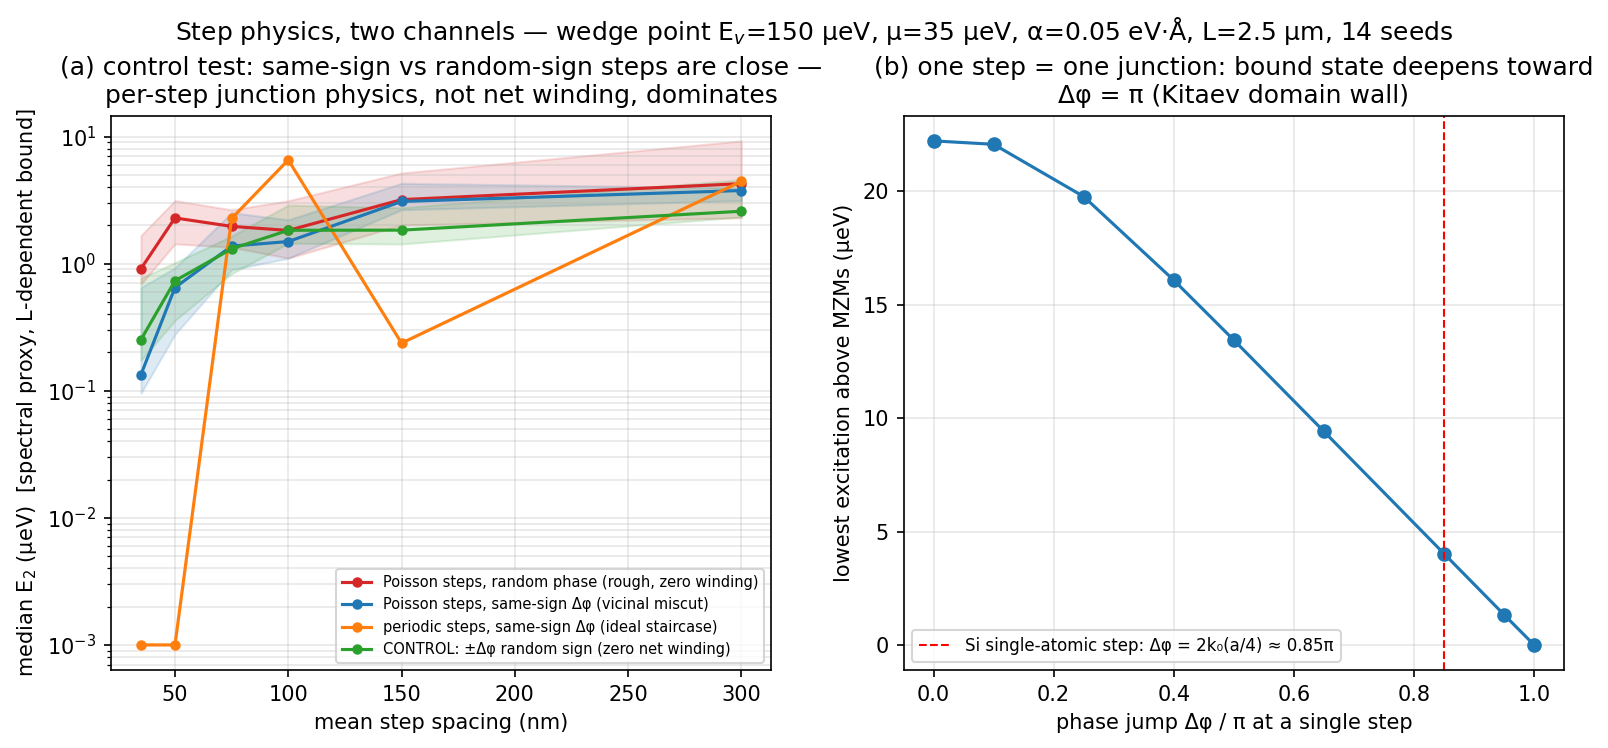
\includegraphics[width=0.95\textwidth]{output/fig9_step_statistics.png}
\caption{Step physics in the inter-valley-paired electron wire. (a)~Controlled
scenario comparison at fixed jump magnitude: same-sign (vicinal) and sign-randomized
(zero-winding control) staircases are statistically indistinguishable---per-step
junction physics, not winding, dominates. (b)~A single VO phase step is a
Josephson-like junction; the Si single-step value $0.85\pi$ sits near the Kitaev
domain-wall point $\pi$.}
\label{fig:steps}
\end{figure}

\section{Valence band}\label{sec:holes}
\subsection{Six-band [110] $k\cdot p$ + Poisson: the primary hole model}
Quasi-1D hole channels in Si FinFETs have measured strong, gate-tunable SOC
\cite{camenzind,voisin,bosco} and anisotropic $g$-tensors \cite{geyer} ---
and every benchmark device is a [110]-oriented channel on a (001) surface.
Our primary hole model is therefore the six-band ($\Gamma_8 \oplus \Gamma_7$)
$k\cdot p$ fin Hamiltonian rotated to the [110] channel, with
self-consistent tri-gate electrostatics available as a control (Supplement
S10; validated against bulk dispersions, the four-band limit to 0.006\%,
and Kramers/Hermiticity to machine precision). It gives a gate-stable
wire-axis $g_{x'} = 1.43$--$1.66$ across all benchmark geometries and the
full field range, $m^* \approx 0.20$, $\alpha$ up to 0.075\,eV\,\AA{}
($l_{so} \approx 50$\,nm), and $g_{y'} = 2.0$--$2.2$ inside the measured
window --- within 0.3--0.6 of the measured along-fin $g \approx 1.9$--2.3,
a residual of the size and sign expected from electrostatic asymmetry
(which raises $g_{x'}$ and $\alpha$ together, Supplement S10.2) and
0.1--0.2\% process strain \cite{venitucci}.

\emph{Pedagogical [100] limit and the covariation caution.} The four-band
hard-wall [100] model that earlier drafts used as primary reproduces
$l_{so} = 32$--101\,nm but illustrates a trap the [110] geometry largely
avoids [Fig.~\ref{fig:lk}]: there, the vertical field that builds $\alpha$
(to 0.054\,eV\,\AA) suppresses the wire-axis $g_x$ from 1.1 to 0.5 while
raising $g_z$ to 2.4--4.2 ($m^* \approx 0.44$, SOC axis in-plane
transverse) --- a harmful $\alpha$--$g$ covariation. Its seven-geometry bracket keeps $g_x \in [0.4, 1.1]$, an apparent
factor-of-two below measurement that the six-band [110] treatment resolves
as predominantly an axes artifact: the split-off band moves $g_x$
\emph{down} (consistent with Ref.~\cite{venitucci}: its envelope weight is
negligible), electrostatics is a $\pm25\%$ geometry-signed correction, and
the [110] rotation closes $\sim$60\% of the gap. All platform numbers
below use the [110] tensors; the frozen [100]/static values are retained
in Supplement S10.3 for provenance.

\begin{figure}[tb]\centering
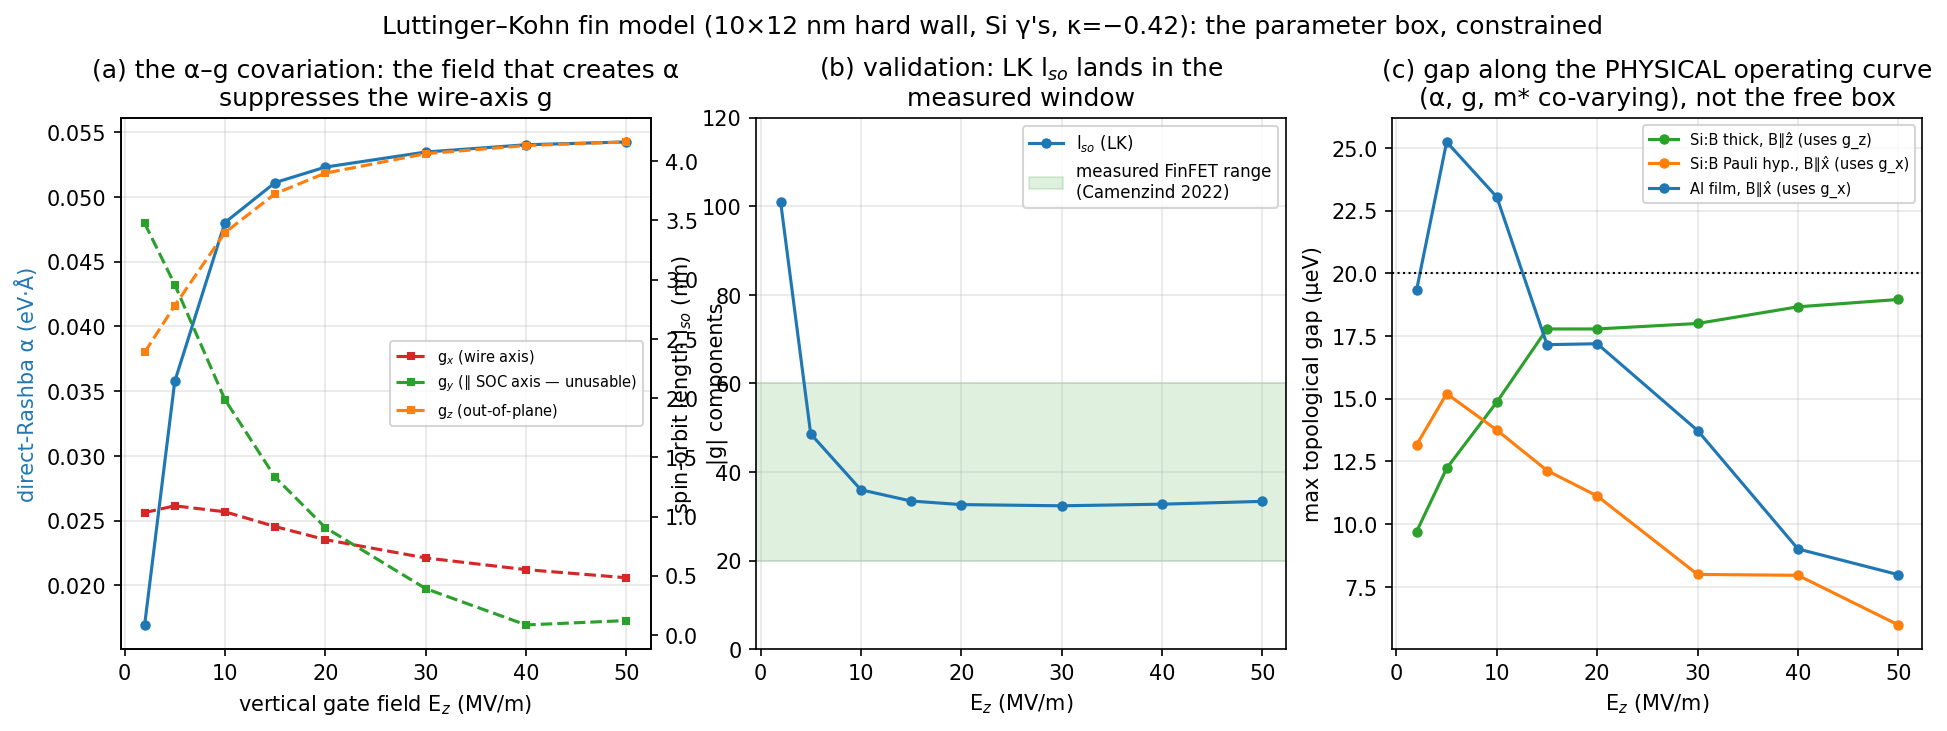
\includegraphics[width=0.95\textwidth]{output/fig10_lk_constraint.png}
\caption{Luttinger--Kohn constraint on the hole platform: (a)~$\alpha$--$g$
covariation under the gate field; (b)~validation of $l_{so}$ against FinFET
measurements; (c)~accessible gap along the physical operating curve for three
parent/orientation scenarios.}
\label{fig:lk}
\end{figure}

\subsection{Parents, orientation, and the surviving designs}\label{sec:parents}
Field-orientation maps [Fig.~\ref{fig:orient}], using the tilted-field
topological criterion of Osca, Ruiz and Serra \cite{osca}, under both
$g$-tensors and two parents give the design rules: (i)~an \textbf{Al film} parent is locked to in-plane fields but
strong---34$\ueV$ metallization-renormalized at the center point, up to
55$\ueV$ bare over orientations (Fig.~\ref{fig:orient}, not
renormalized)---\emph{if} a hard-gap Al/Si-hole
interface can be fabricated (none exists); (ii)~a \textbf{thick Si:B} parent
\cite{bustarret,prb2010,duvauchelle,chiodi2024} is orientation-tolerant and, using only
measured critical fields ($B_{c2} \approx 0.1$--0.4\,T, orbital-limited), supports
10--19$\ueV$ at fields tilted toward out-of-plane (riding $g_z$; the center
point is 11.0$\ueV$ bare / 9.8--10.1 renormalized on finer optimizer grids,
Supplement S5, moves over 8.0--10.6$\ueV$ under $\pm$20\% parent-model
variations, and falls to 7.6$\ueV$ under the dynamic self-energy control of
Sec.~\ref{sec:controls}); the in-plane
wire-axis direction is $g$-starved (3--9$\ueV$). (iii)~The \textbf{thin-film Si:B}
route turns the ``Pauli-limited'' hypothesis into a fabrication target: with coherence
lengths from measured perpendicular critical fields ($\xi = 29$--57\,nm), films of
$d \lesssim 18$--36\,nm have parallel orbital critical fields above the Pauli limit
$B_P = 1.11$\,T, and $d = 10$--20\,nm films support \textbf{21--27$\ueV$}
(modulo unmodeled $T_c(d)$ suppression). Quasiparticle poisoning bounds the role of the
measured-field stack: at operating fields the Si:B parent gap is 29--33$\ueV$, so
$x_{qp} = 10^{-6}$ requires $T_{\rm eff} \le 25$--29\,mK (Al reference: 130\,mK)---a
detection platform, not a parity-coherent qubit, absent parent-gap engineering.
Table~\ref{t:scenario} adjudicates the surviving scenarios at the [110]
parameters with the dynamic self-energy as the central estimate. The [110]
geometry changes the design logic: with $g_{x'} \approx 1.6$ usable
\emph{in-plane along the wire}, film parents no longer need the orientation
compromise, while the measured-field Si:B stack is strongest at tilted
field --- 8.4--10.5$\ueV$ dynamic (Supplement S11.1; the static
12.5--17.1$\ueV$ values are superseded) --- and only marginal in-plane
(3.8--5.3$\ueV$). Tuning tolerances are not the obstacle: the dynamic
optima tolerate $\pm14$--$30\ueV$ in $\mu$, $\gtrsim$35\% in $B$, and a
factor $\ge 3$ in $\Gamma$ (Supplement S11.1). Transport-level validation
passes at the hole operating points exactly as for electrons, 50\,mK
tunneling spectroscopy brackets the true gap to $\pm35\%$, and a
failure-mode library shows the discriminating diagnostic pair is the
scattering invariant co-read with the transport gap (Supplement S11.2).
Multi-subband occupancy and spatially fluctuating coupling $\Gamma(x)$ are
both benign (Supplement S11.5). The decisive negative result is the
charge-trap calibration (Supplement S11.4): oxide-interface charge at
standard densities ($10^{10}$--$10^{11}$\,cm$^{-2}$) produces correlated
potential disorder orders of magnitude beyond the $\sim$25--50$\ueV$ RMS
tolerance, so \emph{interface quality is the gating materials requirement}
for any MOS-style implementation --- favoring remote-doping-free
Si/SiGe-style channels, dramatically better oxides, or metallic-density
screening.

% Tier-based scenario table (round 6): replaces the master table in the main
% text (the frozen master table moved to Supplement S10.3). Columns per the
% review: scenario / demonstrated? / required unproven property / static
% bare / static renorm / dynamic / tier verdict / main failure mode /
% decisive measurement. Numbers: ledger tags platform110, r6_scenarios,
% kp6_110, realism, fig8.qp_poisoning; [110] six-band parameters throughout
% (the experimentally relevant channel orientation).
\begin{table}[tb]\centering
\caption{Scenario adjudication under the operational tiers
(Sec.~\ref{sec:usable}), six-band [110] parameters, dynamic self-energy as
the central estimate (static values are upper bounds).
$^{\dagger}$\,=\,rests on an undemonstrated materials property. All hole
rows additionally inherit the binding oxide-charge constraint of
Supplement S11.4.}
\label{t:scenario}
\resizebox{\textwidth}{!}{%
\begin{tabular}{l l l c c c l l l}
\toprule
scenario & demonstrated? & unproven requirement & \multicolumn{3}{c}{gap ($\ueV$)} &
tier verdict & main failure mode & decisive measurement\\
\cmidrule(lr){4-6}
 & & & bare & renorm. & dyn. & & & \\
\midrule
Si $e^-$ intrinsic & partial (interface) & --- & 1.6 & --- & --- &
FAIL & SOC shortfall & ---\\
Si $e^-$ engineered$^{\dagger}$ & no & $\alpha \approx 0.05$\,eV\,\AA{} in Si;
step control & 29.8 & --- & --- & COND & step yield (2--5\% unaligned;
50--68\% at $\chi \le 10^\circ$) & miscut gap spectroscopy\\
\midrule
Si:B thick (measured), tilted & parent: yes (bulk) & none (measured inputs)
& 12.0--17.1 & 10.3--12.6 & \textbf{8.4--10.5} & S (marginal) &
QP poisoning ($T_{\rm eff} \le 25$--29\,mK); correlated $\mu(x)$ &
device-geometry [110] $g$-tensor\\
Si:B thin film, Pauli$^{\dagger}$ & no & $B_{c\parallel}$ at Pauli limit;
$T_c(d)$ & 21--23 & 16.6--18.7 & \textbf{12.5--13.0} & S$^{\dagger}$
(cond.) & film hypothesis; QP ($\le 29$\,mK) & thin-film
$B_{c\parallel}$\\
Al film$^{\dagger}$ & no & hard-gap Al/Si-hole interface & 36.6--40.5 &
26.0--32.1 & \textbf{16.9--18.4} & S$^{\dagger}$, near-N$^{\dagger}$,
Q$^{\dagger}$ (130\,mK) & interface nonexistent; correlated $\mu(x)$
$\lesssim 25$--50$\ueV$ RMS & interface demonstration\\
\bottomrule
\end{tabular}}
\end{table}


\begin{figure}[tb]\centering
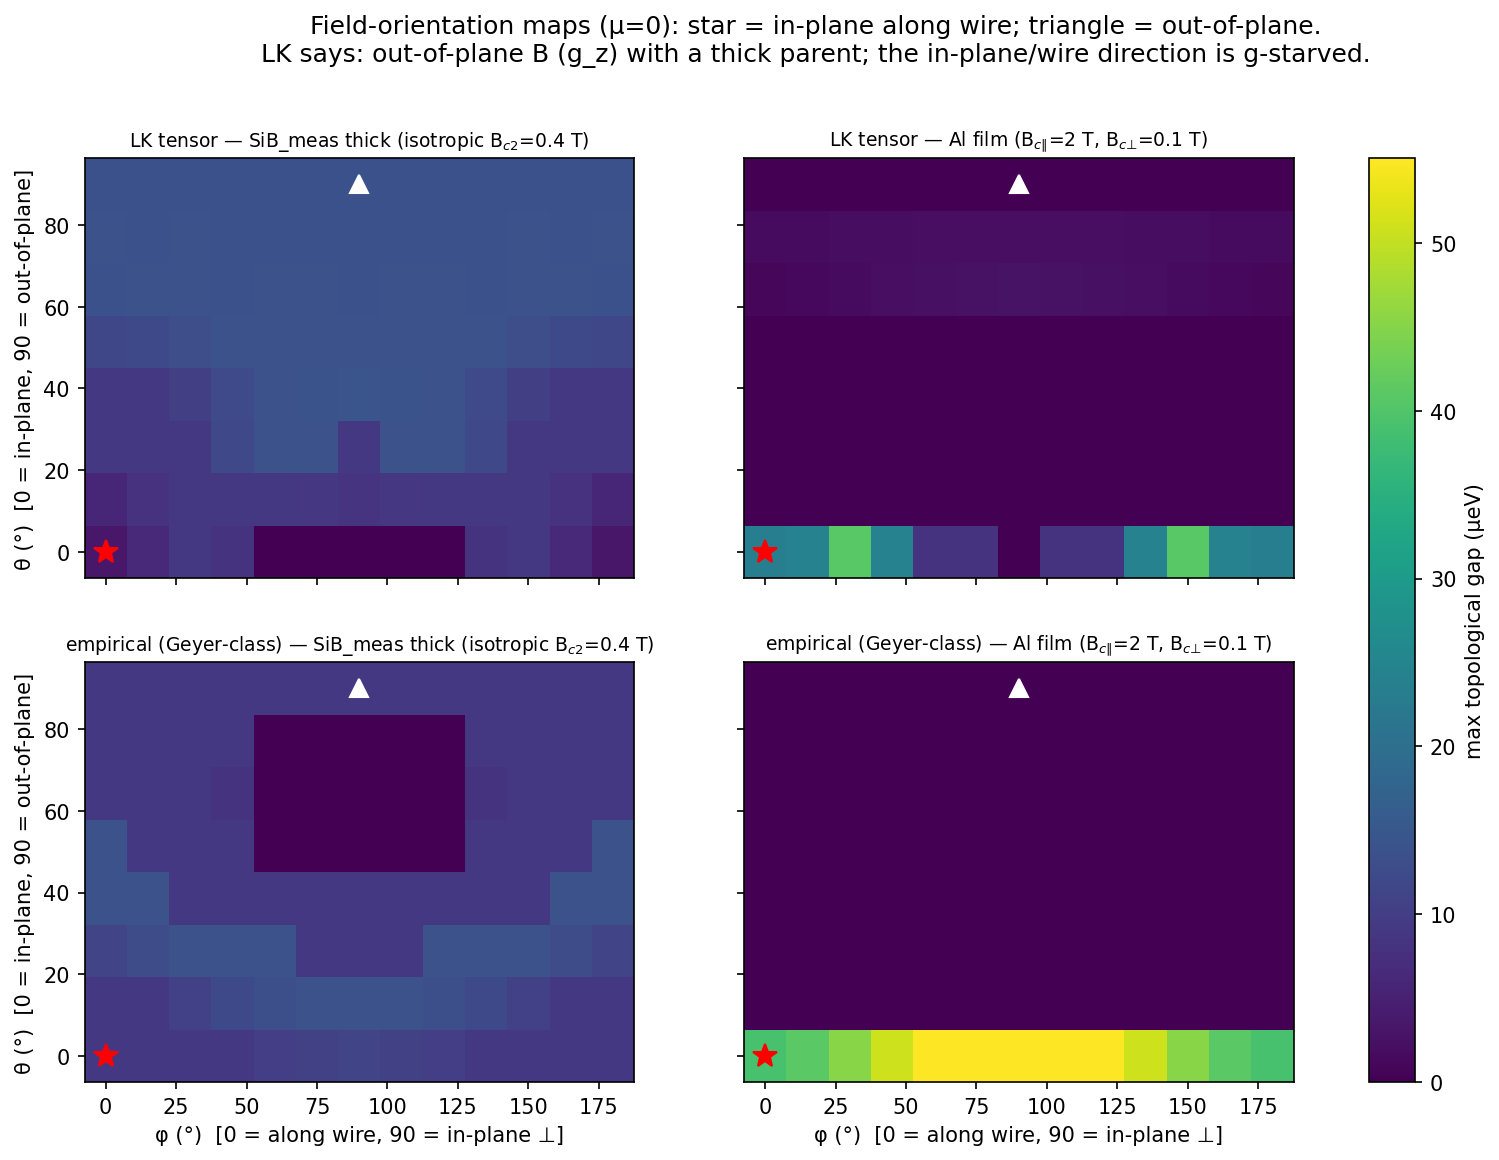
\includegraphics[width=0.92\textwidth]{output/fig11_field_orientation.png}
\caption{Maximum topological gap vs field orientation for LK (top) and empirical
(bottom) hole $g$-tensors, with thick measured-Si:B (left) and Al-film (right)
parents. Star: in-plane along the wire; triangle: out-of-plane.}
\label{fig:orient}
\end{figure}

\begin{figure}[tb]\centering
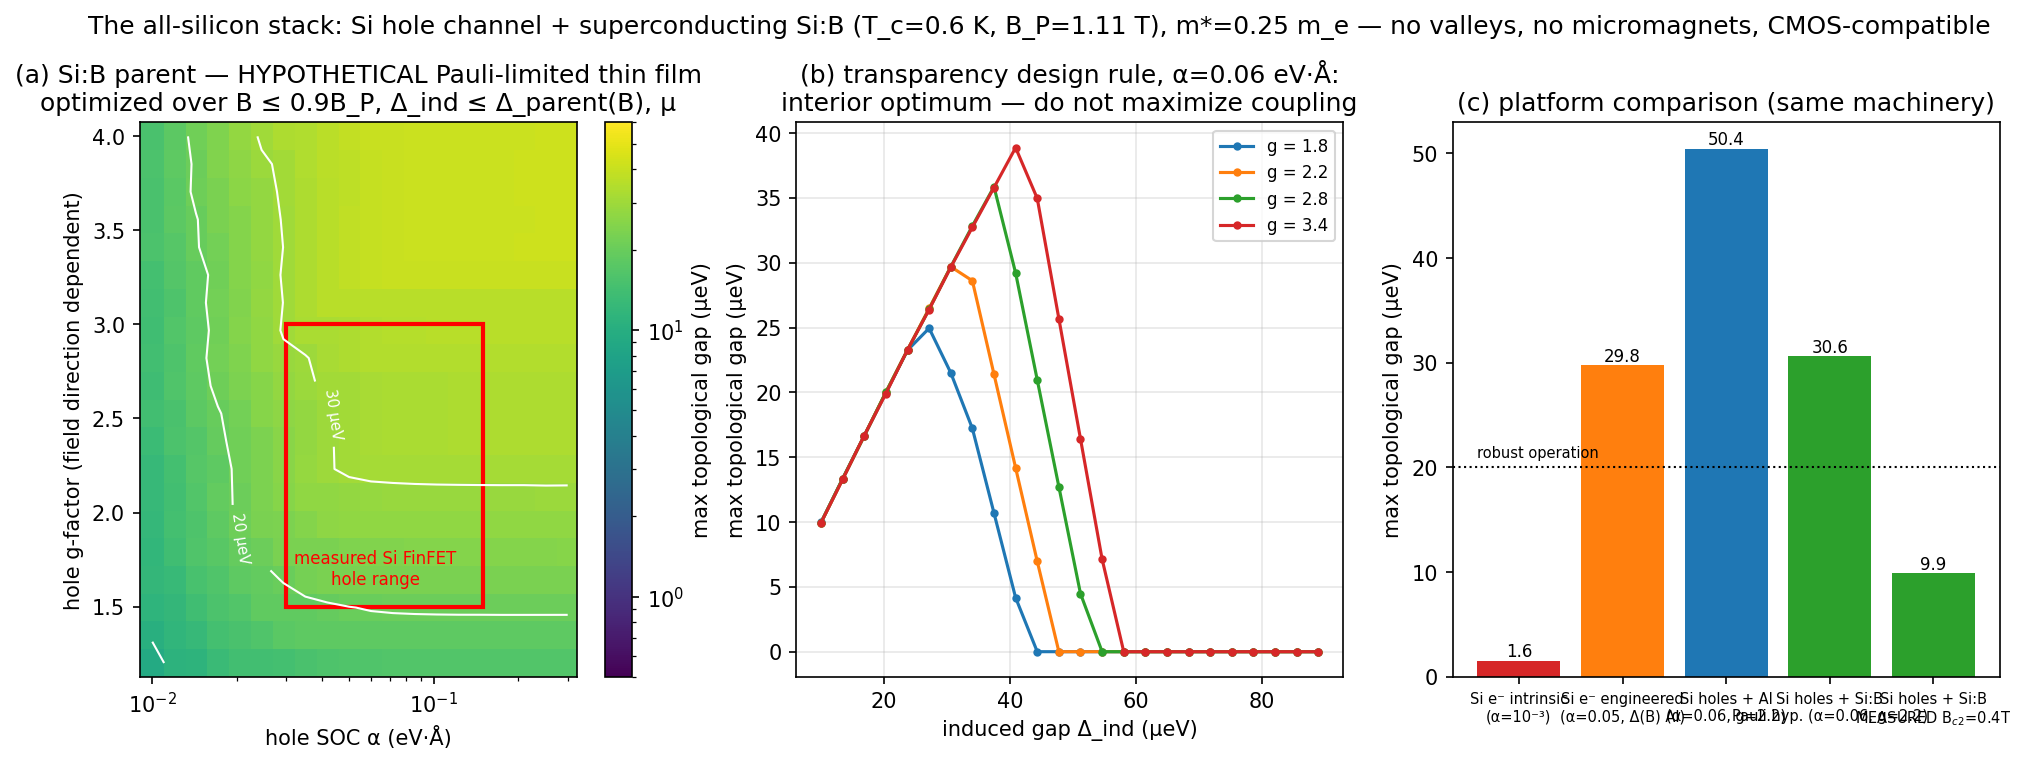
\includegraphics[width=0.95\textwidth]{output/fig8_allsilicon_holes.png}
\caption{The all-silicon stack under the (hypothetical) Pauli-limited Si:B parent:
(a)~gap over the empirical $(\alpha, g)$ box; (b)~the transparency design rule
(interior optimum); (c)~platform comparison including the measured-field Si:B
scenario.}
\label{fig:allsi}
\end{figure}

\section{Transport-level verification}\label{sec:transport}
RGF transmission with normal leads validates the clean wire (transport gap 37.3 vs
bulk 36.8$\ueV$) and provides $\mathrm{sign}\det r$ as a topological invariant. Under
onsite disorder the spectral proxy (third-smallest $|E|$) is \emph{conservative} at
moderate strength (localized states carry no current): the engineered-electron case's
half-gap threshold moves from $W \approx 410$ to $\approx 548\ueV$, and breakdown is
abrupt---a class-D zero-energy transmission anomaly coinciding with invariant sign
flips---rather than a soft closing [Fig.~\ref{fig:transport}]. The same machinery
extended to eight-orbital valley cells yields the Anderson-insulator warning of
Sec.~\ref{sec:valley}.

\begin{figure}[tb]\centering
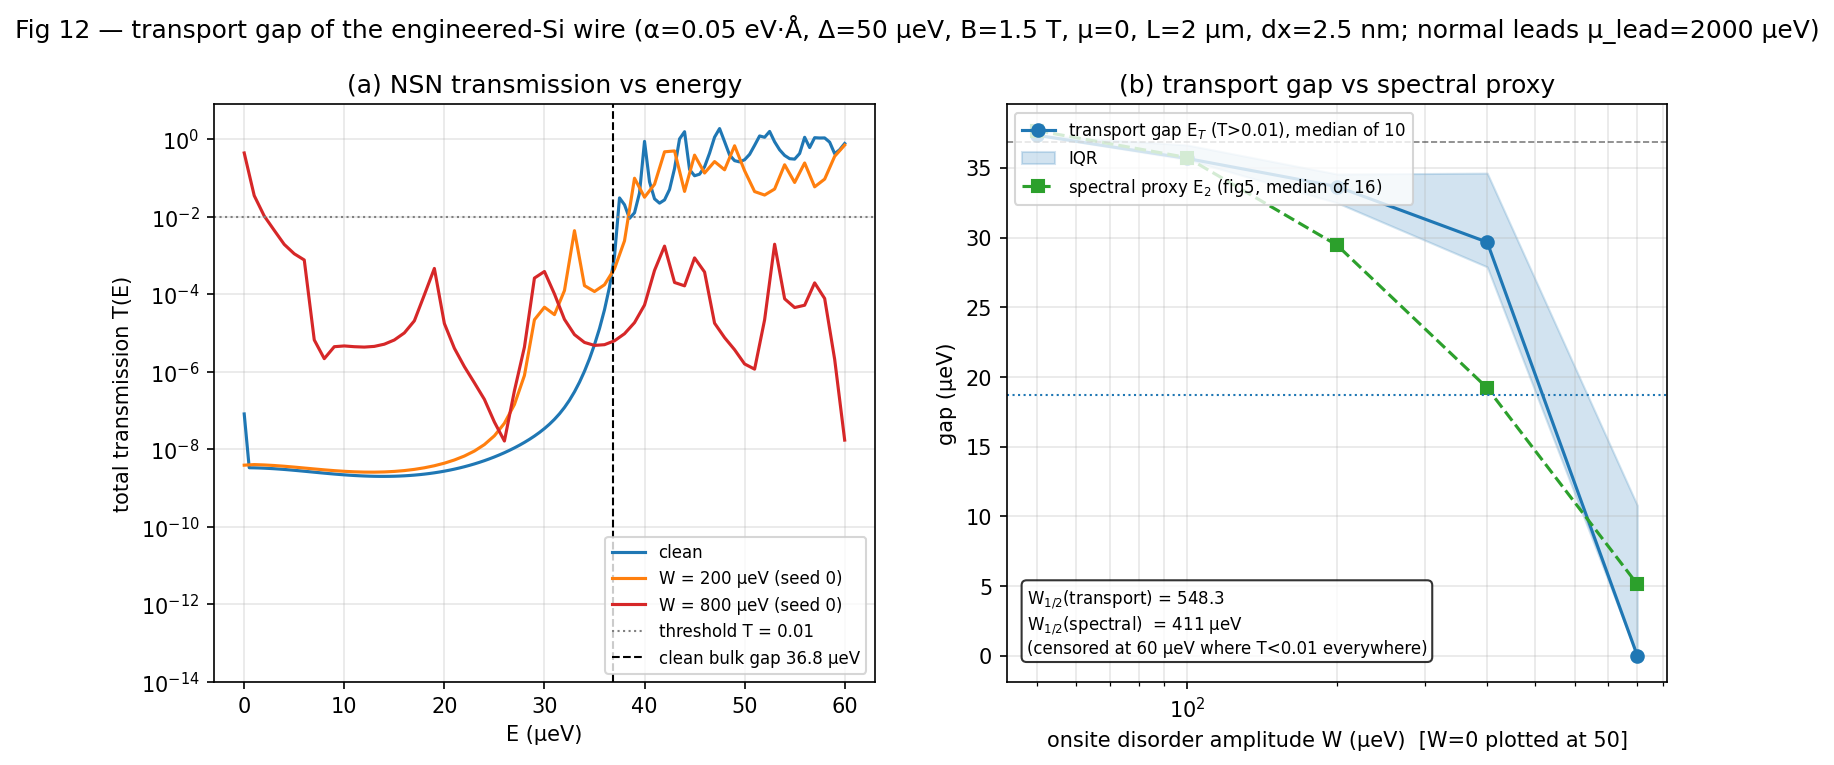
\includegraphics[width=0.9\textwidth]{output/fig12_transport_gap.png}
\caption{Transport vs spectral disorder thresholds (engineered-electron case):
(a)~transmission spectra; (b)~median transport gap vs disorder with the spectral
proxy overlaid.}
\label{fig:transport}
\end{figure}

\section{Realism controls}\label{sec:controls}
Four controls test the headline numbers against the caricatures they rest
on (Supplement S9).
(i)~\emph{Dynamic self-energy}: replacing the static $\Delta$ with the full
$\Sigma(\omega)$ and re-optimizing over tunnel coupling $\Gamma$ gives
center-point gaps of 7.6$\ueV$ (measured Si:B, $\Gamma^* = 10\ueV$),
14.9$\ueV$ (Pauli Si:B, $\Gamma^* = 30$), and 24.2$\ueV$ (Al,
$\Gamma^* = 45$) --- $1.4$--$2.1\times$ below the static bare values and
24--30\% below the static-renormalized ones, which are hereby demoted to
upper bounds; Dynes broadening adds a $\gamma_D/\Delta_p \lesssim 10^{-3}$
requirement for 50\,mK operation. (ii)~\emph{Orbital coupling}: Peierls-phase
controls show $<0.05\%$ gap suppression at fin widths for the tilted Si:B
design --- the orientation maps survive. (iii)~\emph{Pairing-channel mixing}:
intra-valley admixture $\eta$ never weakens the step-junction mechanism
(the step reappears as a pairing-phase junction; $2\times$ deeper bound
state by $\eta^* \approx 0.24$) while healing staircase ensembles --- our
$\eta = 0$ ensembles are conservative, and $\eta \ll \eta^*$ is expected
since intra-valley pairing requires $2k_0$ momentum transfer.
(iv)~\emph{Morphology and correlated disorder}: with miscut-derived terrace
ensembles, device \emph{yield} (25--33\% failure fraction at
0.05--$0.1^\circ$ miscut), not the median gap, is binding; wires along step
edges or step-bunched templates empty the failure tail. Correlated $\mu(x)$
disorder at 50$\ueV$ RMS collapses the hole-platform median gap to
3.5--6.8$\ueV$ where the iid baseline retains 29$\ueV$: smooth
electrostatics is the binding fabrication requirement, and our earlier
iid thresholds overstate robustness by $4$--$8\times$ at fixed RMS.

\section{Discussion}
Two measurements would do the most to settle the silicon question. First, the \textbf{parallel critical
field of thin ($\le$20\,nm) laser-doped Si:B films}: if it approaches the Pauli limit,
as measured coherence lengths permit, the all-silicon hole stack supports
$\gtrsim$20$\ueV$ gaps in a CMOS-compatible, same-crystal materials system; if films
remain orbital-limited at $\sim$0.4\,T, the stack is capped near 10--15$\ueV$ and
detection-only. Second, the \textbf{wire-axis hole $g$-factor and SOC axis} in the
actual gated geometry: our LK bracket and the published FinFET values differ by
$2\times$ along the one direction that matters for film parents. Both measurements are
standard characterization, neither requires a working topological device, and the
electron-side miscut prediction offers a third, independent test of the framework. We
caution that the step-junction mechanism, the orientation maps, and all platform
numbers inherit the stated caricatures (single channel, hard-wall cross
sections, parent-gap models \cite{nijholt}); their domains of validity and the sensitivity of every headline number to them are
quantified in Supplements S5--S6 and S9--S11.

\emph{Relation to Ge-hole platforms.} The closest precedent is
Luttinger--Kohn-based Majorana design for gate-defined Ge hole channels
\cite{gehole}. The silicon case differs in the decisive inputs: a
CMOS-native, same-crystal materials stack with a possible all-silicon
superconducting parent (Si:B); a smaller split-off gap making six-band
treatment mandatory; the [110] FinFET $g$-tensor phenomenology; and, on
the electron side, the conduction-valley step mechanism, which has no Ge
analogue and supplies this paper's sharpest falsifiable prediction.

\emph{What would falsify this study.} (i) Miscut/step-density-resolved gap
spectroscopy on proximitized Si \emph{electron} devices showing induced-gap
hardness independent of step density would falsify the valley-step
mechanism. (ii) A measured device-geometry [110] hole $g$-tensor outside
1.4--2.3, or strongly gate-dependent, would falsify the six-band design
inputs. (iii) Thin-film Si:B with $B_{c\parallel}$ far below the Pauli
limit would eliminate the all-silicon detection scenario. (iv) An Al/Si-hole
interface with a hard induced gap would, conversely, promote the strongest
scenario from hypothetical to testable --- the framework is falsifiable in
both directions.

\section*{Data and code availability}
All figures and quoted numbers regenerate from the committed code
(\texttt{run\_analysis.py}, \texttt{transport.py}, \texttt{transport\_valley.py},
\texttt{lk\_holes.py}, \texttt{qp\_poisoning.py}, \texttt{convergence.py},
\texttt{tests.py}); the numerical ledger is \texttt{output/data/key\_numbers.json},
and per-figure regeneration commands, the environment specification, and seed
families are documented in \texttt{README.md} and Supplement S4/S10. The full
repository --- code, figures, numerical ledger, scan checkpoints, test suite,
review-round corrections log, and this manuscript's source --- is public at
\begin{center}
\url{https://github.com/wtrevena/feasibility-of-creating-majorana-modes-in-silicon-nanowires}
\end{center}
\textbf{Version synchronization:} this manuscript (draft v4), the
Supplement (v4), the repository code, and the numerical ledger are a single
analysis state: the tagged commit recorded in \texttt{MANIFEST.json}, whose
curated map ties every headline number in this paper to its ledger key and
is verified in continuous integration (\texttt{tools/manifest.py --check}).
An archival snapshot (tagged commit and DOI) will additionally be deposited
on Zenodo at submission. [Zenodo DOI: to be inserted at submission.]

\section*{Acknowledgments and provenance}
Analysis, numerical implementation, verification, and manuscript preparation
were assisted by AI agents (Claude, Anthropic) under the author's direction.
Six internal adversarial numerical-review rounds (AI red-team referee-style
reports followed by point-by-point revisions; see \texttt{RESPONSE*.md}) are
documented, with their corrections, in the repository log. AI-assisted review
supplements but does not substitute for the reproducibility materials above;
all claims trace to committed, seeded code. This draft has not yet undergone
human peer review.

\begin{thebibliography}{99}\small
\bibitem{kitaev} A. Kitaev, Phys.-Usp. \textbf{44}, 131 (2001).
\bibitem{lutchyn2010} R. M. Lutchyn, J. D. Sau, S. Das Sarma, Phys. Rev. Lett.
\textbf{105}, 077001 (2010).
\bibitem{oreg2010} Y. Oreg, G. Refael, F. von Oppen, Phys. Rev. Lett. \textbf{105},
177002 (2010).
\bibitem{mourik} V. Mourik \emph{et al.}, Science \textbf{336}, 1003 (2012).
\bibitem{pan2020} H. Pan, S. Das Sarma, Phys. Rev. Research \textbf{2}, 013377 (2020).
\bibitem{aghaee} M. Aghaee \emph{et al.} (Microsoft Quantum), Phys. Rev. B
\textbf{107}, 245423 (2023).
\bibitem{cole2015} W. S. Cole, S. Das Sarma, T. D. Stanescu, Phys. Rev. B \textbf{92},
174511 (2015).
\bibitem{kjaergaard} M. Kjaergaard, K. W\"olms, K. Flensberg, Phys. Rev. B \textbf{85},
020503(R) (2012).
\bibitem{turcotte} S. Turcotte \emph{et al.}, Phys. Rev. B \textbf{102}, 125425 (2020).
\bibitem{micromagnet2025} arXiv:2505.06040 (2025).
\bibitem{losert} M. P. Losert \emph{et al.}, Phys. Rev. B \textbf{108}, 125405 (2023).
\bibitem{hosseinkhani} A. Hosseinkhani, G. Burkard, Phys. Rev. B \textbf{100}, 125309
(2019).
\bibitem{osca} J. Osca, D. Ruiz, L. Serra, Phys. Rev. B \textbf{89}, 245405 (2014).
\bibitem{bosco} S. Bosco, B. Het\'enyi, D. Loss, PRX Quantum \textbf{2}, 010348 (2021).
\bibitem{camenzind} L. C. Camenzind \emph{et al.}, Nat. Electron. \textbf{5}, 178
(2022).
\bibitem{geyer} S. Geyer \emph{et al.}, Nat. Phys. \textbf{20}, 1152 (2024);
arXiv:2212.02308.
\bibitem{venitucci} B. Venitucci, L. Bourdet, D. Pouzada, Y.-M. Niquet,
Phys. Rev. B \textbf{98}, 155319 (2018).
\bibitem{hensel} J. C. Hensel, G. Feher, Phys. Rev. \textbf{129}, 1041
(1963).
\bibitem{voisin} B. Voisin \emph{et al.}, Nano Lett. \textbf{16}, 88 (2016).
\bibitem{bustarret} E. Bustarret \emph{et al.}, Nature \textbf{444}, 465 (2006).
\bibitem{prb2010} C. Marcenat \emph{et al.}, Phys. Rev. B \textbf{81}, 020501(R)
(2010).
\bibitem{duvauchelle} J. E. Duvauchelle \emph{et al.}, arXiv:1508.04075 (2015).
\bibitem{chiodi2024} arXiv:2404.02748 (2024).
\bibitem{reviewSiSC} arXiv:2108.03031 (review).
\bibitem{maier} F. Maier, J. Klinovaja, D. Loss, Phys. Rev. B \textbf{90}, 195421
(2014).
\bibitem{reeg} C. Reeg, D. Loss, J. Klinovaja, Phys. Rev. B \textbf{97}, 165425 (2018).
\bibitem{nijholt} B. Nijholt, A. R. Akhmerov, Phys. Rev. B \textbf{93}, 235434 (2016).
\bibitem{gehole} Phys. Rev. B \textbf{109}, 035433 (2024) (gate-defined Ge
hole nanowires as Majorana platforms).
\end{thebibliography}
\end{document}
